\documentclass{isd}

\usepackage{gensymb}
\usepackage[utf8]{inputenc}
\usepackage[T1]{fontenc}
\usepackage{graphicx}
\usepackage{multirow}
\usepackage{subcaption}

%\graphicspath{{/home/damir/Pictures/}} %if pictures not in current directory of tex file

\begin{comment}
\usepackage[backend=biber, style=numeric, giveninits=true, maxbibnames=99]{biblatex}
\addbibresource{references.bib} % Replace with your .bib file

\DeclareNameFormat{family-given}{%
  \nameparts{#1}%
  \usebibmacro{name:family-given}
    {\namepartfamily}
    {\namepartgiveni} % Use given-name initials
    {\namepartprefix}
    {\namepartsuffix}
  \usebibmacro{name:andothers}}

% Suppressing DOI, ISSN, ISBN from bibliography entries
\DeclareFieldFormat{doi}{}
\DeclareFieldFormat{issn}{}
\DeclareFieldFormat{isbn}{}
  
\DeclareNameAlias{default}{family-given}
\DeclareNameAlias{sortname}{default}
\DeclareFieldFormat[article,book,inbook,inproceedings]{title}{#1}
\renewcommand*{\labelnamepunct}{\addcolon\space}
\end{comment}

\usepackage{etoolbox}
\appto{\bibsetup}{\setlength{\itemsep}{0pt}}




\newcommand{\mj}[2]{#1\hspace*{1.5pt}#2}

\begin{document}

\title{Using the ARMADA Algorithm to Analyze Physiological Marker Patterns in Presumed Emotional States}

%\author[Author et al.]{Paweł Mańczak, Teresa Zawdadzka}

%\email{pawelmanczak14@gmail.com, teresa.zawadzka@pg.edu.pl}

%\institution{Gdańsk University of Technology, Faculty of Electronics, Telecommunications and Informatics}

%\city{Gdańsk, Gdańsk}

%\country{Poland, Poland
\maketitle
\vspace{-2.7cm}

\begin{abstract}
%Affective computing has emerged as a pivotal field in bridging the gap between human emotional intelligence and machine responsiveness, focusing on the computational modeling and automatic recognition of human emotions. This study aims to investigate the feasibility of detecting sequential patterns of physiological transitions during presumed emotional episodes. To achieve this, the ARMADA algorithm is utilized to analyze datasets characterized by continuous annotations and synchronized cardiovascular and electrodermal features as well as skin temperature. The study successfully validated the selection of the ARMADA algorithm for temporal pattern discovery. The generated association rules were proven to be statistically significant through the application of a permutation test, ensuring that the discovered relationships were not the result of random chance. Despite the inherent variability across the different datasets, 54 specific rules met the rigorous criteria for cross-dataset validation, demonstrating their consistency and reliability. Furthermore, a quantitative analysis of these rules yielded significant findings regarding the predominance of moderate affective states and HRV synchronicity, as well as the identification of psychological lag through transition logic. Notably, the analysis also uncovered a unique temporal association between low-arousal states and electrodermal activity, providing deep insights into the physiological markers of emotional transitions. 
Affective computing bridges the gap between human emotions and machine responsiveness through computational modeling. This study investigates detecting sequential patterns of physiological transitions during emotional episodes using the ARMADA algorithm. By analyzing datasets with synchronized cardiovascular, electrodermal, and skin temperature features, the study validated ARMADA’s effectiveness for temporal pattern discovery. The generated association rules were proven statistically significant via permutation tests, with over 50 rules meeting rigorous cross-dataset validation criteria. Quantitative analysis revealed significant findings regarding the predominance of moderate affective states, HRV synchronicity, and psychological lag in transition logic.\par\vspace*{2mm}
\textbf{Keywords:} Physiological Rule Mining, Emotion Recognition, ARMADA Algorithm, Affective Computing, Cross-Dataset Analysis
\end{abstract}

\section{Introduction}
Automatic emotion recognition plays a crucial role in Affective Computing, offering the potential for continuous assessment of human emotional states \cite{sharma2019dataset}. Emotion recognition systems are built on diverse modalities, most notably facial expressions. Still, researchers have long also recognized the potential of physiological signals for emotion assessment. This stems from the fact that unlike facial expressions or voice, physiological responses such as Electrodermal Activity (EDA), Photoplethysmography (PPG), and skin temperature (SKT) are largely controlled by the autonomic nervous system and reflect genuine emotional states without conscious distortion \cite{shu2018review}. In recent years, an extensive body of literature has adopted machine learning and deep learning techniques, including Support Vector Machines (SVMs), Convolutional Neural Networks (CNNs), and Recurrent Neural Networks such as LSTMs, to process these complex time-series signals \cite{bota2019review}. Although these models often achieve strong classification performance, their predictions are typically difficult to interpret in mechanistic terms, making it challenging to explicitly explain how temporally evolving physiological changes relate to the emergence of a particular emotional state. 

From another perspective, the past few years have highlighted the necessity of shifting emotion recognition systems away from 'black box' models toward architectures that enable explainability of their outputs \cite{gunning2016xai, adadi2018peeking}. Despite the abundance of modern Explainable AI (XAI) techniques, rule-based systems have seen a resurgence in importance due to their naturally transparent and self-explanatory nature \cite{a18090586, rahman2026axai}. The application of sequential rule mining to physiological signals, all the while, remains in its infancy. Even though human physiological responses naturally unfold over time, very few studies actually use sequential rules to analyze them \cite{schneider2025associations}. To address this gap the research objective is to \textbf{explore the feasibility of discovering temporal patterns within specific physiological signals, leveraging continuously annotated data through the application of the Association Rule Mining And Discovery Algorithm (ARMADA)} \cite{winarko2007armada}. 

%To achieve the goal, firstly, the research questions were defined in Section \ref{sec:researchQuestions}. Subsequently, a literature review is conducted in Section \ref{sec:relatedWork}. Section \ref{sec:methodology} details the research methodology, while the subsequent sections follow this defined methodology directly, addressing the data acquisition (Section \ref{sec:datasets}), experimental design (Section \ref{sec:experimentalDesign}) and implementation (Section \ref{sec:experimentsImplementation}), as well as the analysis of the results (Section \ref{sec:experimentsResults}). The final Section \ref{sec:conclusions} concludes the study by summarizing the key findings and outlining directions for future work.

%Research studies frequently rely on sophisticated architectures capable of high-accuracy classification. However, while these predictive models demonstrate impressive performance, they predominantly function as black-box mechanisms, rarely offering transparent insights into how temporal interactions among distinct physiological events shape human emotions over time.

%through physiological signals . While numerous scientific works have successfully extracted temporal and sequential rules to model emotions, these efforts have predominantly focused on text data, such as social media posts and blogs \cite{skenduli2021mining, wen2014emotion, giuntini2021tracing}, or video data \cite{porhet2017mining}.\par

%Surprisingly, the application of sequential rule mining to physiological signals remains virtually unexplored. Even though human physiological responses naturally unfold over time, very few studies actually use sequential rules to analyze them. Instead, modern research frequently relies on machine learning and deep learning architectures to process physiological time-series data, including Support Vector Machines (SVMs), Convolutional Neural Networks (CNNs), and Recurrent Neural Networks such as LSTMs. Although these models often achieve strong classification performance, their predictions are typically difficult to interpret in mechanistic terms, making it challenging to explicitly explain how temporally evolving physiological changes relate to the emergence of a particular emotional state \cite{bota2019review, shu2018review}.\par

\section{Research Questions}
\label{sec:researchQuestions}

To provide a structured investigation to achieve the primary objective of this study, the two research questions were defined:

\textbf{RQ1: Technical Feasibility and Rule Stability}
\textit{To what extent can the ARMADA algorithm effectively extract stable and statistically significant temporal association rules from multi-modal, continuously annotated physiological datasets?},

{\textbf{RQ2: Pattern Discovery and Physiological Correlation} \textit{Which specific temporal patterns in physiological signals (such as HRV and EDA) are most frequently associated with transitions in emotional states according to the discovered rules?} and

{\textbf{RQ3: Multimodality} \textit{How does the performance and interpretability of multi-modal association rules compare to single-modal rules in describing emotional transitions?}

Due to the complexity of the first research question, the supportive sub-questions were defined and investigated: RQ1.1 (Annotation Source) \textit{How does the source of emotional labels—specifically self-reports versus expert external annotations—influence the quality and consistency of the discovered temporal rules?}} and RQ1.2 (Emotional Model) \textit{To what extent does the choice of emotional model (discrete categories \cite{ekman1992argument} vs. multidimensional valence-arousal space \cite{russell1980circumplex}) affect the algorithm's ability to identify meaningful patterns in physiological signals?}
%For the analysis of the generalizability of the patterns addressed in RQ2, the three sub-questions were formulated: RQ2.1 (Demographic Factors) \textit{To what extent do demographic characteristics, specifically gender and age, influence the structure and types of temporal association rules extracted by the ARMADA algorithm?}, RQ2.2 (Cross-group Consistency) \textit{Are there identifiable "universal" physiological patterns that remain consistent across different demographic groups, or are the discovered rules predominantly group-specific?}, and 

%To address this gap, this paper introduces a sequential rule mining approach to physiological data, shifting the focus from opaque "black-box" predictions to interpretable temporal rules. Specifically, this study aims to answer the following research questions:

%\begin{enumerate}
%    \item Are there universal temporal patterns in which changes in physiological signals precede changes in emotional states (arousal, valence)?
%    \item Do temporal rules work bidirectionally (physiology $\rightarrow$ emotions and emotions $\rightarrow$ physiology), or does one direction dominate?
%    \item Do the extracted temporal patterns differ between genders?
%    \item Does age affect the discovered physiological rules?
%    \item Which temporal rules extracted by the ARMADA algorithm remain stable regardless of the experimental context?
%    \item Do multimodal rules (combining EDA, HRV, and HR simultaneously) exhibit higher confidence than unimodal rules?
%\end{enumerate}


\section{Related Work}
\label{sec:relatedWork}

%\subsection{Emotion Recognition and Physiological Signals}
%The field of Affective Computing has long recognized the potential of physiological signals for emotion assessment. Unlike facial expressions or voice, physiological responses such as Electrodermal Activity (EDA), Photoplethysmography (PPG), and Heart Rate Variability (HRV) are largely controlled by the autonomic nervous system and reflect genuine emotional states without conscious distortion \cite{shu2018review}. In recent years, an extensive body of literature has adopted machine learning and deep learning techniques to process these complex time-series signals \cite{bota2019review}. StThe past few years have highlighted the necessity of shifting emotion recognition systems away from 'black box' models toward architectures that allow for the explainability of their outputs. Studies frequently rely on sophisticated architectures capable of high-accuracy classification. However, while these predictive models demonstrate impressive performance, they predominantly function as black-box mechanisms, rarely offering transparent insights into how temporal interactions among distinct physiological events shape human emotions over time.

The presented study is aligned with the broader trend in affective computing of integrating XAI to enhance model transparency. Among the leading approaches in this field are Attention-Based, Generative-Based, and Graph-Based XAI methods \cite{10130818}. The body of research encompasses both single-modality analyses \cite{ai7030095, 10766406} and multimodal frameworks \cite{11170860}.

In relation to the subject of this work, the second important branch consists of studies that map multimodal physiological manifestations to underlying cognitive processes. Among these, the most recent study by Machhi, Vilas et al. (2026) \cite{Machhi2026} is of particular importance. In this context, there are also studies searching for rules describing the influence of the single modalities on human affect, e.g. \cite{HRV2025}.

However, the studies most closely related to this work are those addressing the application of sequential pattern mining to emotion recognition. Still, these solutions have been mostly restricted to modalities other than biosignals. A significant amount of research has focused on extracting sequential emotion-aware rules from text data, particularly social media content and micro-blogs \cite{skenduli2021mining, wen2014emotion}. Similarly, sequential pattern mining has been utilized to analyze multimodal combinations of verbal and facial clues in video data, unearthing temporal patterns during interpersonal interactions \cite{porhet2017mining}. Despite these advancements across text and video modalities, physiological data remains notably excluded from sequential rule-mining approaches, leaving an unaddressed gap regarding the explicit, universally interpretable temporal rules defining human physiological reactions.
%For instance, tracing the temporal emotional roadmap of users through sequences of online posts has proven valuable in depressive tendency detection \cite{giuntini2021tracing}. Similarly, sequential pattern mining has been utilized to analyze multimodal combinations of verbal and facial clues in video data, unearthing temporal patterns during interpersonal interactions \cite{porhet2017mining}. Despite these advancements across text and video modalities, physiological data remains notably excluded from sequential rule-mining approaches, leaving an unaddressed gap regarding the explicit, universally interpretable temporal rules defining human physiological reactions.

\section{Methodology}
\label{sec:methodology}

This section outlines the research framework, starting with the fundamental assumptions that guide the analysis of physiological responses to emotional stimuli as well as core methodology.%, both depicted in Figure \ref{fig:methodology}. 

%\begin{figure}[!h]
%\centering
%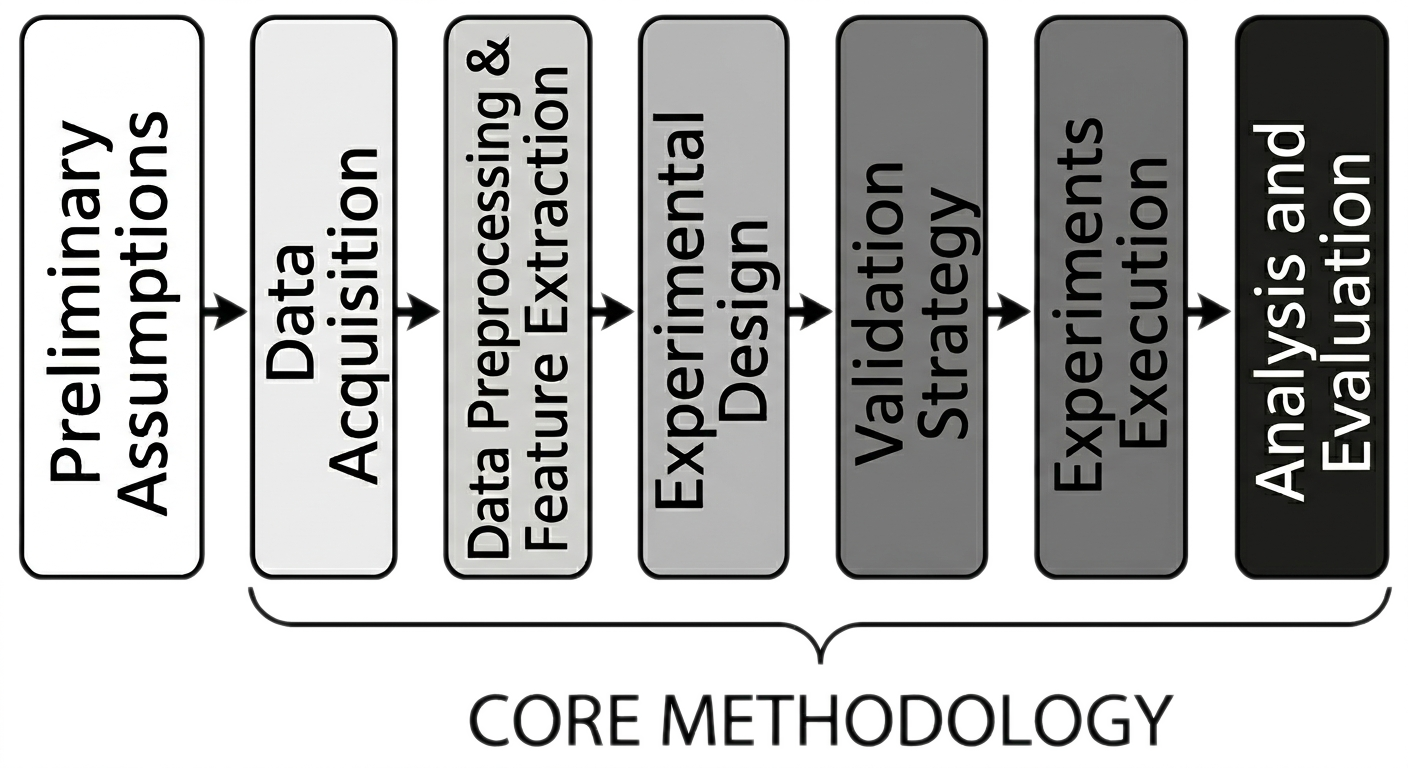
\includegraphics[width=0.3\textwidth]{Methodology_1.png}
%\caption{Research methodology applied in the study.}
%\label{fig:methodology}
%\end{figure}

\subsection{Preliminary Assumptions}
To ensure the clarity and focus of the investigation, the primary assumptions and technical choices have been established.

\textbf{Selection of Physiological Modalities:} The study focuses on three primary types of signals: Blood Volume Pulse (BVP), EDA, and SKT. These modalities were selected for two main reasons. First, they are highly sensitive to autonomic nervous system changes, providing reliable markers for emotional arousal (EDA \cite{jang2014relationship, sharma2016brief}, BVP \cite{park2022photoplethysmogram, jang2014relationship, shu2018review} and SKT \cite{4462012}) and valence (primarily Heart Rate Variability (HRV) \cite{porges2007polyvagal, shaffer2017overview, appelhans2006heart}). Second, they represent the most prevalent biosignals in publicly available affective computing datasets, ensuring that the proposed framework is compatible with a wide range of existing research benchmarks and allows for cross-dataset validation of the discovered rules.

\textbf{Pattern Discovery Paradigm:} The research framework is based on the Sequential Association Rules (SAR) mining approach. In contrast to static association rules, SAR accounts for the temporal order of events, which is essential for capturing the dynamic nature of emotional transitions and the inherent physiological lag between a stimulus and the body's response.

\textbf{Algorithmic Framework:} The pattern discovery process utilizes the ARMADA algorithm, engineered to extract association rules from multi-modal time-series data. Instead of raw continuous points, it relies on discretized symbolic intervals, enabling the integration of heterogeneous signals (e.g., high-frequency cardiac data and slow-varying EDA) into a unified event stream. By representing physiological changes as time-stamped symbols, ARMADA identifies complex temporal predicates—such as overlaps, contains, or starts—that extend beyond simple co-occurrence. This is essential for modeling the physiological lag between emotional stimuli and autonomic responses. Furthermore, the algorithm avoids rigid a priori structures, detecting both acute spikes and long-term trends. The resulting human-readable "If-Then" rules ensure transparency, aligning with the XAI paradigm by providing causal-like justifications for affective state classifications.

%The pattern discovery process is executed using the ARMADA algorithm, which is specifically engineered to extract association rules from multi-modal time-series data. A fundamental characteristic of this approach is its reliance on discretized symbolic intervals \cite{winarko2007armada} rather than raw continuous data points. This methodology enables the seamless integration of signals with heterogeneous characteristics, such as high-frequency cardiac data and slow-varying EDA, by transforming them into a unified stream of interval-based events. By representing physiological changes as time-stamped symbols with a defined duration, ARMADA facilitates the identification of complex temporal predicates—such as \textit{before}, \textit{meets}, \textit{overlaps}, \textit{is-finished-by}, \textit{contains}, \textit{equals}, and \textit{starts} — that extend beyond simple co-occurrence. This capability is essential for modeling the physiological lag inherent between an emotional stimulus and the subsequent autonomic nervous system response. Furthermore, the algorithm does not impose a rigid, a-priori structure on the discovered rules, allowing for the detection of both acute signal spikes and long-term correlational trends. The resulting set of human-readable "If-Then" rules ensures total model transparency, directly aligning with the XAI paradigm by providing causal-like justifications for affective state classifications.

\textbf{Rule Evaluation Metrics:} To assess the quality and reliability of the discovered patterns, the research framework relies on standard association rule metrics—primarily \textit{Support}, \textit{Confidence}, and \textit{Lift}—specifically adapted for temporal sequences.



%\subsection{Sequential Association Rule Mining}
%Sequential rule mining is a specialized data mining framework aimed at discovering temporal associations between events in sequence databases. \cite{fournier2011rulegrowth,fournier2014erminer} Unlike standard association rule mining (e.g., Apriori \cite{huang2000fast}), which identifies co-occurring items regardless of order, sequential rule mining extracts patterns of the form $X \rightarrow Y$, implying that the antecedent event $X$ temporally precedes the consequent event $Y$. Sequential pattern mining algorithms, such as GSP (Generalized Sequential Pattern) \cite{srikant1996mining} or PrefixSpan \cite{han2001prefixspan}, focus on discovering frequent subsequences and are often used as baselines or building blocks for rule extraction.\par


%\textit{Support} quantifies the prevalence or frequency of a rule across the entire dataset. It is defined as the proportion of sequences in $S$ where the event $X$ is followed by the event $Y$:
%\begin{equation}
%Support(X \rightarrow Y) = \frac{|\{s \in S \mid X \mbox{ precedes } Y \mbox{ in } s\}|}{|S|}
%\end{equation}

%\textit{Confidence} measures the directional reliability of the rule, defined as the conditional probability that $Y$ will follow $X$, given that $X$ has already occurred:
%\begin{equation}
%Confidence(X \rightarrow Y) = \frac{Support(X \rightarrow Y)}{Support(X)}
%\end{equation}

%In the context of physiological emotion recognition, defining strict bounds for these metrics alongside explicit temporal gaps is crucial to ensure that physiological reactions are not arbitrarily linked to temporally distant emotion states.


%\subsubsection{Selection of the ARMADA Algorithm}

%Selecting an appropriate data mining algorithm for this study required matching the specific nature of our dataset with the algorithm's technical capabilities. Specifically, the chosen method had to support multiple data channels simultaneously, integrate both categorical variables (e.g., participant sex) and continuous numerical values (e.g., EDA signals), and, most importantly, capture strict time consequences between physiological events and emotional responses.


%Although some temporal rule-mining approaches can operate without an explicit discretization step \cite{zhao2021tsarm}, this is not problematic in our setting, as ARMADA is designed for discretized interval-based events \cite{winarko2007armada}. This representation is also consistent with the nature of the analyzed features, which are subject-specific and normalized before rule extraction, making their transformation into discrete states both natural and interpretable.

%Moreover, ARMADA is able to represent several types of temporal relationships between interval-based events, including \textit{before}, \textit{meets}, \textit{overlaps}, \textit{is-finished-by}, \textit{contains}, \textit{equals}, and \textit{starts} \cite{winarko2007armada}. Thus, the relation between two events is not limited to a simple ordering such as \(A\) before \(B\), but can also capture more specific temporal configurations between intervals. This is useful in physiological emotion recognition, where the association between a physiological response and an emotional state may depend not only on event order, but also on the exact temporal relation between them. In addition, the \texttt{MAXGAP} parameter makes it possible to constrain the maximum allowable delay between related events, focusing the rule discovery process on temporally local dependencies \cite{winarko2007armada}.


\subsection{Core Methodology}

The six main steps are defined within the Core Methodology. The first one, \textbf{Data Acquisition}, involves selecting datasets that address the research questions—specifically those providing continuous annotations and multimodal biosignals. Additionally, it is required that some datasets contain self-annotations, whereas others provide external ones. A specific emotional model is not mandatory, as it was assumed that discrete models could be transformed into multidimensional ones and vice versa. Incorporating that requirement carried a risk with respect to the availability of the dataset; however, the study requires at least two externally annotated sets and two self-annotated sets. In the \textbf{Data Preprocessing and Feature Extraction} step, physiological signals are processed to extract key features, which are then subjected to normalization and discretization. This stage also involves the harmonization of labeling across disparate datasets. Depending on the specific emotional model employed, appropriate transformations are applied to unify the emotion representation. A key component of this research involves the \textbf{Experimental Design and Validation Strategy}, which establishes the protocols required to investigate the research questions. In the subsequent \textbf{Experiments Execution} phase, these designs are implemented and validated. Finally, the resulting data are analyzed to evaluate their alignment with the study's original goal and research questions (\textbf{Analysis and Evaluation}).

\section{Data Acquisition}
\label{sec:datasets}

Searching for datasets combining multimodal physiological recordings with relatively continuous or densely sampled emotions annotations was conducted in an unstructured study, which encompassed analysis of the Systematic Literature Review (SLR) \cite{ometov2025stress, 11214492, app14167165}, interviews with other Affective Computing researchers, and direct efforts to obtain dataset access, including contacting dataset authors with formal requests, completing User Agreement Forms when required, and, in the case of the EMBOA dataset, reaching out to the person responsible for the project.
%[tutaj proszę o uzupełnienie co tam jeszcze Pan robił, aby te zbiory danych pozyskać]. 
As a result of this study, five multimodal emotion datasets were chosen: K-emoCon \cite{park2020k}, Continuously Annotated Signals of Emotion (CASE) \cite{sharma2019dataset}, Continuous Physiological and
Behavioral Emotion Annotation Dataset for 360\degree Videos (CEAP-360VR) (hereinafter referred to as CEAP) \cite{xue2021ceap}, EMBOA \cite{barkan2024challenges}, and EmoWorker \cite{lee2026multimodal}. These datasets differ in both acquisition setting and annotation protocol, covering controlled laboratory recordings as well as conversational and immersive VR scenarios. They also include both self-reported annotations and externally assigned labels, which makes them suitable for evaluating rule mining under heterogeneous emotion-labeling schemes.

More specifically, EMBOA was collected in a human-robot interaction setting and combines Empatica E4 peripheral signals with externally assigned behavioral annotations (done with variable frequency), whereas K-emoCon captures dyadic conversations and provides self, partner, and external affective ratings (done every 5 seconds) alongside physiological recordings. CASE represents a controlled laboratory dataset with high-resolution physiological signals and continuous self-assessment gathered using a joystick interface (with frequency 20 Hz), while CEAP extends this paradigm to immersive \(360^\circ\) audiovisual stimulation in virtual reality \cite{xue2021ceap} (with annotation frequency equals to 10 Hz). EmoWorker, in turn, provides multimodal physiological recordings acquired in a workplace-related context together with continuous affect annotations \cite{lee2026multimodal} with a frequency ranging from 5 to 10 Hz.
In each dataset (except EMBOA), the number of participants was approximately 30 (+/-2). For the EMBOA dataset, the number of participants was 16.
The datasets further vary in the physiological modalities and sampling rates they provide. In addition to the physiological signals selected for this study, some datasets also incorporate electrocardiogram, electroencephalogram, respiration, eye tracking, or motion-related signals \cite{park2020k,sharma2019dataset,xue2021ceap,lee2026multimodal}. For all datasets (except CASE) the frequency of BVP is 64Hz, and 4Hz for EDA and SKT. The frequency of all three signals for CASE is 1000Hz. 
%The annotation schemes and modalities used in the evaluated datasets and incorporated in the study are summarized in Table \ref{tab:datasets}.

% Please add the following required packages to your document preamble:
% \usepackage{multirow}
%\begin{table}[]
%\caption{Annotation schemas and modalities used in the incorporated datasets.}
%\label{tab:datasets}
%\begin{tabular}{l|lll|lll}
%\multicolumn{1}{c|}{\multirow{2}{*}{\textbf{Dataset}}} &
%  \multicolumn{3}{c|}{\textbf{Annotations}} &
%  \multicolumn{3}{c}{\textbf{Frequency (Hz)}} \\ \cline{2-7} 
%\multicolumn{1}{c|}{} &
%  \multicolumn{1}{c|}{\textbf{Type}} &
%  \multicolumn{1}{c|}{\textbf{Origin}} &
%  \multicolumn{1}{c|}{\textbf{Frequency (Hz)}} &
%  \multicolumn{1}{c|}{\textbf{BVP}} &
%  \multicolumn{1}{c|}{\textbf{EDA}} &
%  \multicolumn{1}{c}{\textbf{SKT}} \\ \hline
%EMBOA &
%  \multicolumn{1}{l|}{External} &
%  \multicolumn{1}{l|}{BORIS} &
%  Variable &
%  \multicolumn{1}{l|}{64} &
%  \multicolumn{1}{l|}{4} &
%  4 \\ \hline
%K-emoCon &
%  \multicolumn{1}{l|}{\begin{tabular}[c]{@{}l@{}}External\\ Partner\\ Self\end{tabular}} &
%  \multicolumn{1}{l|}{} &
%  0.2 &
%  \multicolumn{1}{l|}{64} &
%  \multicolumn{1}{l|}{4} &
%  4 \\ \hline
%CASE &
%  \multicolumn{1}{l|}{Self} &
%  \multicolumn{1}{l|}{Joystick} &
%  20 &
%  \multicolumn{1}{l|}{1000} &
%  \multicolumn{1}{l|}{1000} &
%  1000 \\ \hline
%CEAP-360VR &
%  \multicolumn{1}{l|}{Self} &
%  \multicolumn{1}{l|}{\begin{tabular}[c]{@{}l@{}}Self-assesment\\ Questionnaire\end{tabular}} &
%  10 &
%  \multicolumn{1}{l|}{64} &
%  \multicolumn{1}{l|}{4} &
%  4 \\ \hline
%EmoWorker &
%  \multicolumn{1}{l|}{Self} &
%  \multicolumn{1}{l|}{Continuous traces} &
%  5-10 &
%  \multicolumn{1}{l|}{64} &
%  \multicolumn{1}{l|}{4} &
%  4
%\end{tabular}
%\end{table}

%To facilitate a unified comparative analysis and enable the ARMADA-based rule mining process, data from all disparate sources was resampled, synchronized, and aligned into standardized 5-second multi-resolution time windows.\par

%The common modalities used in the cross-dataset analysis were EDA, BVP, and skin temperature (SKT). These signals were selected because they are available in most of the analyzed datasets and provide some information about autonomic aspects of emotional responses.

%Electrodermal activity (EDA) reflects changes in skin conductance driven mainly by sympathetic nervous system activation \cite{jang2014relationship}. For this reason, EDA is one of the physiological modalities most consistently associated with arousal \cite{jang2014relationship, sharma2016brief}.

%Blood Volume Pulse (BVP) is a pulse-related physiological signal derived from photoplethysmography \cite{li2021pulse}, from which features such as heart rate (HR), inter-beat interval (IBI), and heart rate variability (HRV) can be estimated. HRV features include, for example, SDNN, RMSSD, and pNN50 \cite{kolakowski2025comparative}. In the literature, BVP-derived features are more consistently associated with arousal than with valence \cite{park2022photoplethysmogram, jang2014relationship, shu2018review}.

%Skin temperature (SKT) is a peripheral physiological measure influenced by blood flow in the skin and autonomic nervous system activity. In emotion research, it is treated mainly as an indirect marker of autonomic arousal \cite{salazar2015mental}. 

\section{Data Preprocessing and Feature Extraction}
As it was already stated in Section \ref{sec:datasets}, the datasets contain either self-annotations or external ones. In the case of the K-emoCon dataset, it contains both types of annotations, therefore to ensure unambiguous characteristics (only one type of annotation) for each dataset, it is divided into two separate ones - one set for self-annotations and one for external ones (hereinafter referred to as K-emoCon and K-emoCon (ext), respectively). As a result, the input for further processing is actually 6 datasets.

Physiological features were extracted directly from the raw signals of all datasets using the same NeuroKit2-based processing pipeline \cite{makowski2021neurokit}, ensuring a standardized representation across modalities and datasets before temporal segmentation.
HR-based features were used to characterize both the instantaneous cardiac state and short-term HRV. In particular, HR and IBI represented the current dynamics of heart activity, whereas \texttt{hrv\_rmssd}, \texttt{hrv\_pnn50}, \texttt{hrv\_sdnn}, \texttt{hrv\_cvnn}, and \texttt{hrv\_hfn} quantified variations between successive beats and reflected autonomic cardiovascular regulation. EDA features were included to capture phasic electrodermal responses, with \texttt{eda\_scr\_amp}, \texttt{eda\_scr\_auc}, and \texttt{eda\_peaks} describing the magnitude and occurrence of skin conductance reactions. Temperature features comprised \texttt{temp\_mean} and \texttt{temp\_slope}, representing the average thermal level within a segment and its temporal trend, respectively.

%\subsection{Sliding Window Mechanism}
To synchronize disparate sampling rates across multiple datasets, continuous physiological signals and ground truth annotations were segmented using a static sliding window mechanism. A multi-resolution methodology tailored to modality reactivity parameters was applied; dynamic signals were extracted utilizing 5-second sliding windows \cite{boucsein2012electrodermal}. Conversely, parameters inherently reliant on longer macroscopic measurement phases, specifically HRV and SKT, were captured via independent 30-second windows \cite{rossi2020error}. After this process, the combined dataset from all 6 datasets consists of 176 sets (one for each participant and a few additional ones due to more than one recording for few participants in EMBOA dataset) with the average rounded number of timestamped events equal to 2485 (CASE), 85 (CEAP), 524 (EMBOA), 1233 (EmoWorker), 667 (K-emoCon), and 672 (K-emoCon (ext)).    

%\subsection{Discretization of Physiological Features}
Because ARMADA requires symbolic input, continuous physiological signals were discretized into three states: Low (L), Medium (M), and High (H). To reduce subject-specific bias, since physiological baselines and response ranges can differ markedly across individuals \cite{gutierrez2024personalized, braithwaite2013guide}, we first applied participant-wise min-max normalization and then defined L/M/H using global terciles computed from the pooled normalized data.
%\subsection{Normalization and Discretization of Emotional Labels}
For datasets featuring native dimensional annotations (e.g., 1--9 Self-Assessment Manikin scales), arousal and valence values were normalized to a $[0, 1]$ range per dataset and divided into strict terciles: low ($[0, 0.33)$), medium ($[0.33, 0.66)$), and high ($[0.66, 1.0]$). This translation successfully yielded $1489$ valid valence timestamped events and $952$ unified arousal timestamped events. In the combined dataset, it resulted in 7265 events for valence (\textit{low} - 1111, \textit{medium} - 4728, \textit{high} - 1426) and 12319 events for arousal (\textit{low} - 1281, \textit{medium} - 4546, \textit{high} - 1502) suitable for ARMADA processing.

To enable dimensional vs. discrete comparisons, all dimensional data were mapped into a $3 \times 3$ grid of 9 categorical emotions via Russell's circumplex model. Combinations of arousal and valence terciles defined unique discrete states (e.g., \textit{high} arousal and valence yielded \textit{excited}; \textit{medium} states yielded \textit{neutral}) \cite{russell1980circumplex}. This synchronized all datasets---both inherently dimensional and dimensional-mapped discrete cohorts (EMBOA)---into a single 9-label framework. Across all datasets, this produced $4073$ \textit{neutral} tuples, followed by \textit{calm} ($947$), \textit{content} ($938$), \textit{alert} ($603$), \textit{stressed} ($603$), \textit{upset} ($553$), \textit{excited} ($484$), \textit{sad} ($304$), and \textit{relaxed} ($207$).

%\subsection{Temporal Alignment of Ground Truth Annotations}
To enable strict association rule mining, annotation streams recorded at varied frequencies or by multiple observers were aggregated into a singular ground truth label per temporal window. For self-reported datasets (e.g., CASE, K-emoCon), high-frequency or asynchronous ratings within a physiological window were simply averaged (linear mean) to yield one synchronized dimensional label. For externally annotated datasets featuring multiple observers, independent ratings were fused into a consensus sequence before window aggregation. For K-emoCon (ext), we used the dataset's native \textit{aggregated\_external\_annotations}, where up to five continuous rating streams were aggregated via majority voting (see Code Availability). In EMBOA, the native percentage agreement across multiple BORIS raters served as the proportional weight mapping categorical emotions onto Russell’s dimensional space. This ensured deterministic emotion tracking across all cohorts.

%\subsection{Age Cohort Unification}
%To support demographic pattern extraction without overly fragmenting the subset populations, participant ages from all 121 (achieved only from self-annotated datasets) analyzed subjects were unified into a balanced binary threshold rather than multiple narrow buckets. Participants were strictly divided into \textit{Young} (age $\leq 25$; 60 participants) versus \textit{Older} (age $> 25$; 61 participants) groupings. Within these participants there are 50 females and 71 males.
%\subsection{Handling Missing Values}
Corrupted intervals and missing values were inherently filtered or marked natively by the original dataset providers, allowing our methodology to bypass artificial interpolation entirely.


\section{Experimental Design}
\label{sec:experimentalDesign}

To achieve the answers to the research questions, the two experiments were defined: Experiment 1 for RQ1, and Experiment 2 for RQ2 and RQ3. 

The experimental pipeline for \textbf{Experiment 1} follows a two-tier approach. Initially, temporal association rules are extracted independently for each of the six datasets to capture site-specific patterns. To evaluate the cross-dataset robustness of the ARMADA algorithm, a consensus-based validation framework is applied. By identifying the common temporal rules across six datasets, the focus is set on patterns that achieve a high level of agreement (consensus) between different experimental setups (specific for each dataset). The resulting discrete sequential rule sets were evaluated using dynamic intersections—gradually escalating from discovering generic rules shared between any two datasets, up to generating rules for the combined datasets being the union of two, three, four, or five datasets (intersecting the rules with the one not included in the combined dataset), utilizing leave-one-out apporach ("one" meaning the whole dataset). To evaluate generic cross-dataset feasibility independently of rigid dataset-specific constraints, a universal minimum support parameter of 30\% (\textit{Minsup = 0.3}) is strictly applied across this foundational phase. This threshold is set due to the assumption that mining patterns in biosignals belongs to the class of mining rare events.

The setup supports two iterations, which vary with the emotion models applied. The first one utilizes the valence-arousal model, and the second one, the uniform discrete 9-label framework.

The datasets with self-reported annotations are strictly isolated from external annotations to prevent structural overlap. To quantify the overlap between the rule sets extracted from the self- and externally-annotated, the Jaccard Similarity Coefficient is employed. This metric provides a normalized measure of the intersection between two sets of rules, accounting for variations in the total number of rules discovered across datasets. This analysis is done only for the valence-arousal model, as it is originally used in most of the incorporated datasets.

 %To measure explicit pattern variations between exclusively self-reported and exclusively external sequences for valence-arousal dimensional inputs. This emotion model was chosen due to its application in experimental framework for all but one (EMBOA) dataset. The last fourth, iteration asesses the structural impact of utilizing dimensional emotion representation versus discrete framework across identical self-reported sequences and relates to RQ 1.2. 



%To validate ARMADA's applicability, input sequences were structured  participant-level multivariate time series combining cardiovascular and EDA signals with synchronized emotional states. We strictly isolated self-reported from external annotations to prevent structural overlap. To evaluate generic cross-dataset feasibility independently of rigid dataset-specific constraints, a universal minimum support parameter of 30\% (\textit{Minsup = 0.3}) was strictly applied across this foundational phase.

%This setup supported three comparative iterations:
%\begin{itemize}
%    \item \textbf{Global Feasibility (RQ1):} Extraction of universal rules across all pooled datasets utilizing the uniform discrete 9-label emotional framework.
%    \item \textbf{Annotation Source (RQ1.1):} Measuring explicit pattern variations between exclusively self-reported and exclusively external sequences, mapped identically on dimensional ($V/A$) inputs.
%    \item \textbf{Emotional Model (RQ1.2):} Assessing the structural impact of utilizing dimensional ($V/A$) representations versus discrete frameworks across identical self-reported sequences.
%\end{itemize}
%\subsection{Experiment 2: Independent Dataset Pattern Discovery}
%To establish dataset-level physiological footprints, the baseline ARMADA methodology was executed independently across each distinct dataset environment using purely dimensional ($V/A$) configurations. To measure cross-compatibility, the resulting discrete sequential rule sets were evaluated using dynamic intersections—gradually escalating from discovering generic rules shared between any two datasets, up to rigid matrices tracking intersections across three, four, or five environments. Datasets possessing dual annotations (e.g., K-emoCon) were treated as independent algorithmic entities during the pairing processes.

%\subsection{Experiment 2: Universal Intersections (RQ2)}
\textbf{Experiment 2} dedicated to RQ2 is built upon the Experiment 1. Building on the results of the initial phase, Experiment 2 is designed to evaluate and interpret the outcomes of Experiment 1 in a broader context. Rather than conducting a separate procedural study, this phase focuses on a deep qualitative analysis of the most reliable association rules identified previously. These high-confidence rules are scrutinized for their functional significance and their practical implications for emotion recognition within the field of affective computing. Furthermore, to address RQ3, the analysis specifically investigates the distribution and roles of the physiological modalities involved. No dedicated experiment is designed for RQ3. 

%To verify cross-group correlational consistency (RQ2.1 and RQ2.2), the fully established temporal patterns derived from universal self-reported dimensional datasets were deeply segmented utilizing the unified global demographic markers (Gender and Age groups). ARMADA was subsequently deployed to isolate specific sequential anomalies fundamentally tied to physiological demographic divergences rather than experimental noise.
% The  of the , a strict universal rule analysis was executed identically across two distinct structural groupings to verify core physiological stability: firstly, intersecting the discrete temporal outputs exclusively derived from the four self-annotated datasets to identify global psychophysiological rules universally present across self-aware environments; secondly, isolating the intersection between the two externally annotated datasets to search for patterns universally perceptible by third-party observers. In both cases the support was not set to strict value, as for the rare events the support is much lower ten 50\% (as in Experiment 1) or the threshold is dynamically set depending on the participants or contexts \cite{380415, inproceedings}. The same assumption was applied in \textbf{Experiment 3}. To verify cross-group correlational consistency, the fully established temporal patterns derived from universal self-reported dimensional datasets were deeply segmented utilizing the unified global demographic markers (Gender and Age groups). ARMADA was subsequently deployed to isolate specific sequential anomalies fundamentally tied to physiological demographic divergences rather than experimental noise.

%The separate experiment was not designed for the RQ3, as the resulting rules achieved within Experiment 2 and 3 were analysed with respect to the modalities utilized in the rules.

In addition to the consensus-based validation framework, permutation tests were conducted to rigorously assess the statistical significance of the discovered patterns. For the first experiment, these tests were utilized to evaluate the magnitude of rule reduction, ensuring that the filtering process effectively isolates non-stochastic associations. Regarding the second and third experiments, the permutation approach served to verify whether significant rules—previously identified through performance metrics—could still be detected within shuffled datasets. This contrastive analysis demonstrates that the validated rules are not artifacts of random data arrangements but represent genuine physiological dependencies.



%\begin{itemize}
%    \item \textbf{Self-Reported Universality:} Intersecting the discrete temporal outputs exclusively derived from the four self-annotated datasets to identify global psychophysiological rules universally present across self-aware environments.
%    \item \textbf{External Universality:} Isolating the intersection between the two externally annotated datasets to search for patterns universally perceptible by third-party observers.
%\end{itemize}

%\subsection{Experiment 4: Demographic Correlational Stability (RQ2.1 \& RQ2.2)}
%To verify cross-group correlational consistency, the fully established temporal patterns derived from universal self-reported dimensional datasets were deeply segmented utilizing the unified global demographic markers (Gender and Age groups). ARMADA was subsequently deployed to isolate specific sequential anomalies fundamentally tied to physiological demographic divergences rather than experimental noise.

\section{Execution of Experiments}
\label{sec:experimentsImplementation}

%The ARMADA algorithm was executed independently on six physiological datasets to address the research questions defined in Section~\ref{sec:researchQuestions}. Four datasets employ \textit{self-annotations} (participants rate their own emotions): CASE ($N = 30$), K-emoCon ($N = 28$), CEAP-360VR ($N = 32$), and EmoWorker\_v2 ($N = 31$). Two datasets employ \textit{external annotations} (observers rate participants' emotions): K-emoCon (ext) ($N = 28$, same physiological data as K-emoCon) and EMBOA ($N = 16$, BORIS-based categorical annotations mapped to arousal/valence via Russell's circumplex model). 

To execute the experiments, a proprietary implementation of the ARMADA algorithm was developed in Python. The experiments were conducted on a MacBook Pro equipped with an Apple M1 chip and 16 GB of unified memory. All experiments presented in this section were conducted, and the reported results were obtained, using scripts available in the public repository \cite{}. The repository contains the implementation necessary to reproduce the experimental procedure and the obtained outcomes.

To assess the technical feasibility of temporal rule extraction from physiological, the ARMADA algorithm was applied to all six datasets under identical strict parameters: $minsup = 0.3$, $minconf = 0.5$, $maxgap = 5$~s, and $max\_pattern\_size = 4$. These settings universally retain only temporal rules that span up to 4 events, constrain events within a 5-second maximum gap, and appear in at least 30\% of the participants with at least 50\% confidence. The semantic filters were applied to ensure cross-modal relevance: rules
containing only BVP/HRV/HR-related or only EDA-related states were rejected, as were rules
linking exclusively physiological modalities without any emotional dimension (arousal or
valence), and rules involving only a single feature type.

%\subsection{RQ1.1: Annotation Source Comparison}
%\label{sec:exec_rq11}
To investigate the influence of annotation source on rule quality, the rules extracted from all four self-annotated datasets were pooled (union) and compared against the pooled rules from both externally annotated datasets. %Additionally, a controlled comparison was performed on K-emoCon, where the same physiological recordings are available with both annotation types, isolating the effect of annotation perspective from physiological differences.

%To assess the impact of the emotional model on pattern discovery, all six datasets were processed under two distinct label representations with the same strict parameters. In the \textit{dimensional} variant, arousal and valence were discretized into three levels (low, medium, high) and used directly as ARMADA events. In the \textit{discrete} variant, arousal and valence were jointly mapped onto a $3 \times 3$ grid to produce nine categorical emotion labels based on Russell's circumplex model \cite{russell1980circumplex}: \textit{stressed}, \textit{alert}, \textit{excited}, \textit{upset}, \textit{neutral}, \textit{content}, \textit{sad}, \textit{calm}, and \textit{relaxed}. Each dataset's native arousal/valence scale was normalized to $[0, 1]$ before mapping.

\section{Results of Experiments}

\label{sec:experimentsResults}
As stated in the experimental design, the base model for experiments is a multidimensional one, so all results are discussed with reference to it unless otherwise noted.

%\subsection{RQ1: Technical Feasibility and Rule Stability}
\textbf{Experiment 1.} ARMADA extracted between 929 and 3032 semantically filtered cross-modal rules per dataset (see Table \ref{tab:rq1_feasibility} for details), capturing diverse temporal relations (\textit{meets}, \textit{before}, \textit{starts}, \textit{equals}) between physiological features and emotional dimensions. The permutation tests, involving the randomization of event sequences, resulted in a substantial rule reduction ranging from 72\% to 97\% across all datasets; this underscores the fact that the vast majority of patterns discovered in the original data are not mere products of event frequency, but are fundamentally dependent on the specific temporal order and causal structure of the physiological signals.

\begin{table}[]
\caption{Metrics for filtered rules extracted with ARMADA per dataset.}
\label{tab:rq1_feasibility}
\begin{tabular}{l|l|l|l|l|l|l}
 &
  \textbf{CASE} &
  \textbf{K-emoCon} &
  \textbf{CEAP} &
  \textbf{EmoWorker} &
  \textbf{\begin{tabular}[c]{@{}l@{}}K-emoCon\\ (ext)\end{tabular}} &
  \textbf{EMBOA} \\ \hline
  \textbf{Dimension Model}  & 2432   & 1208   & 3032   & 929    & 1633   & 2972 \\
\textbf{Discrete Model}       & 643   & 144   & 485   & 171   & 324   & 1184
\\ \hline
\textbf{\begin{tabular}[c]{@{}l@{}}Dimension Model\\ (shuffled)\end{tabular}} &
  82 &
  44 &
  498 &
  50 &
  114 &
  808 \\
\textbf{Reduction} & 96,6\% & 96,4\% & 83,6\% & 94,6\% & 93,0\% & 72,8\%
\\ \hline
\textbf{\begin{tabular}[c]{@{}l@{}}Discrete Model\\ (shuffled)\end{tabular}} &
  38 &
  23 &
  91 &
  20 &
  34 &
  492 \\
\textbf{Reduction} & 94.1\% & 84.0\% & 81.2\% & 88.3\% & 89.5\% & 58.4\%
\\ \hline
\textbf{Ratio}                                                       & 0.26 & 0.12 & 0.16 & 0.18 & 0.20 & 0.40
\end{tabular}
\end{table}

Intersection analyses revealed the algorithm's capacity to discover stable physiology--emotion interactions despite heterogeneous experimental protocols. Figure~\ref{fig:combined_heatmaps} visualizes shared rule generalization. In heatmap (c) of Figure~\ref{fig:combined_heatmaps}, the pairwise overlapping between datasets is depicted. The highest overlapping occurs between CASE and EmoWorker (306 shared rules) and between CASE and K-emoCon (ext) (295 shared rules), while EMBOA shows the least overlapping with other datasets (7--43 shared rules); still, this dataset is for autistic children--a fact possibly influencing the obtained result, yet not incorporated as a variable in the research.
%It is important to remember that this dataset is for autistic children, which can influence the obtained results (this variable is not incorporated in the research).
The next three heatmaps ((a), (b), (d)) show, respectively, pairwise generalization (persistence in a third dataset), triplet generalization (persistence in a fourth dataset), and quadruplet analysis (persistence in a fifth dataset). The results of quintuplet analysis are not presented as no common rules were obtained. Based on the premise that the validity of a pattern increases with its prevalence across multiple independent datasets, and applying the 'majority rule' (consensus in at least four out of six datasets), 1+1+2+54 rules were identified as potentially generalized patterns (depending on the datasets, in which they are approved). However, it is important to exercise caution in this classification; since two of the confirming datasets were derived from the same dataset (K-emoCon), the assumption of total independence is not fully met for the 54 rules. Despite this constraint, these rules still demonstrate a high level of credibility. Furthermore, a significant number of rules were confirmed across three datasets. These are categorized as domain-robust patterns, as they exhibit substantial resilience to environmental changes and suggest strong reproducibility within similar experimental contexts. 

\begin{figure}[thb!]
    \centering
    % --- Row 1 (Pairwise Gen i Triplet Gen) ---
    \begin{subfigure}[b]{0.45\textwidth}
        \centering
        
\includegraphics[width=\textwidth]{figures/heatmap_pairs_generalization_sparse.png}
        \caption{Pairwise Generalization}
        \label{fig:heatmap:pairs_gen}
    \end{subfigure}
    \hfill
    \begin{subfigure}[b]{0.45\textwidth}
        \centering
        
\includegraphics[width=\textwidth]{figures/heatmap_triplets_generalization_sparse.png}
        \caption{Triplet Generalization}
        \label{fig:heatmap:triplets_gen}
    \end{subfigure}

    \vspace{1em} 

    % --- Row 2 (Shared Rules i Quadruplet Gen) ---
    \begin{subfigure}[b]{0.35\textwidth}
        \centering
        
\includegraphics[width=\textwidth]{figures/heatmap_shared_rules.png}
        \caption{Pairwise Shared Rules}
        \label{fig:heatmap:shared}
    \end{subfigure}
    \hfill
    \begin{subfigure}[b]{0.6\textwidth}
        \centering
        
\includegraphics[width=\textwidth]{figures/heatmap_quadruplets_generalization_sparse.png}
        \caption{Quadruplet Generalization}
        \label{fig:heatmap:quads_gen}
    \end{subfigure}

    \caption{Shared rule generalization}
    \label{fig:combined_heatmaps}
\end{figure}


%\subsection{RQ1.1: Influence of Annotation Source}
%\label{sec:results_rq11}

To assess the influence of annotation source (\textbf{RQ1.1}), the union of all rules from the four self-annotated datasets (7095 unique rules) was compared with the union from the two externally annotated datasets (4598 unique rules). A Jaccard similarity of 0.038 (432 shared rules) reveals a relatively small overlap, suggesting that while a core set of physiology--emotion patterns exists, the vast majority of findings are heavily influenced by the annotation paradigm. %Table~\ref{tab:annotation_overview} summarizes the cross-paradigm comparison.

%\begin{table}[!h]
%\small
%\centering
%\caption{Cross-paradigm comparison: self-annotated vs.\ externally annotated rule sets.}
%\label{tab:annotation_overview}
%\begin{tabular}{|l|c|}
%\hline
%\textbf{Metric} & \textbf{Value} \\
%\hline
%Total unique self rules (4 datasets) & 7095 \\
%\hline
%Total unique external rules (2 datasets) & 4598 \\
%\hline
%Shared rules & 432 \\
%\hline
%Self-only rules & 6663 \\
%\hline
%External-only rules & 4166 \\
%\hline
%Jaccard similarity & 0.038 \\
%\hline
%\end{tabular}
%\end{table}



%In a controlled comparison on K-emoCon (identical physiological data), with external annotations yielded more rules then with self-annotations (1633 vs.\ 1208, $J=0.033$). Among the 91 shared rules, external annotations consistently showed higher confidence. Table~\ref{tab:annotation_shared} lists the rules with the largest confidence shifts. These results suggest external annotations produce more consistent, higher-confidence rules, particularly for HRV$\rightarrow$valence associations (confidence reaching 1.000). Self-annotations, however, better captured certain emotion$\rightarrow$EDA associations, hinting at higher sensitivity to interoceptive arousal. Nevertheless, the 432 rules globally shared across paradigms demonstrate that ARMADA extracts a core foundation of generalized patterns independent of annotation source.

%\begin{table}[!h]
%\small
%\centering
%\caption{K-emoCon shared rules with the largest confidence differences between annotation sources.}
%\label{tab:annotation_shared}
%\resizebox{\textwidth}{!}{
%\begin{tabular}{|p{7cm}|c|c|c|c|c|}
%\hline
%\textbf{Rule} & \textbf{Conf} (self) & \textbf{Lift} (self) & \textbf{Conf} (ext) & \textbf{Lift} (self) & \textbf{Conf $\Delta$} \\
%\hline
%hrv\_sdnn\_low $\Rightarrow$ meets valence\_med & 0.500 & 0.500 & 1.000 & 1.000 & +0.500 \\
%\hline
%hrv\_cvnn\_low $\Rightarrow$ meets valence\_med & 0.522 & 0.522 & 1.000 & 1.000 & +0.478 \\
%\hline
%hrv\_cvsd\_low $\Rightarrow$ meets valence\_med & 0.545 & 0.545 & 1.000 & 1.000 & +0.455 \\
%\hline
%hrv\_rmssd\_low $\Rightarrow$ meets valence\_med & 0.565 & 0.565 & 1.000 & 1.000 & +0.435 \\
%\hline
%valence\_med $\Rightarrow$ is-finished-by eda\_high & 1.000 & 1.000 & 0.533 & 0.533 & $-$0.467 \\
%\hline
%\end{tabular}
%}
%\end{table}




%\subsection{RQ1.2: Influence of Emotional Model}
%\label{sec:results_rq12}

As part of Experiment 1, regarding \textbf{RQ1.2}, the rules extracted for the dimensional model and the discret model were compared (see Table~\ref{tab:rq1_feasibility}) across all six datasets. The rules were filtered analogically to the dimensional model, i.e., only cross-modal rules linking an emotional component to a physiological signal were retained. The discrete model produced fewer cross-modal rules in every dataset, yielding only 12--40\% of the dimensional model's rule count. The largest reduction was observed for self-annotated K-emoCon (144 vs.\ 1208 rules; ratio = 0.12), whereas the smallest gap appeared in EMBOA (1184 vs.\ 2972; ratio = 0.40). Across all six datasets, the dimensional model produced 12,206 filtered rules, while the discrete model produced 2,951, corresponding to an overall ratio of 0.24. These results indicate that the dimensional representation preserves a substantially richer set of cross-modal emotion--physiology patterns, whereas the discrete representation leads to a stronger reduction in retained rules and a sparser cross-modal structure. Intersection analyses for a discrete model do not provide the identification of generalized patterns. Approximately 30 domain-robust patterns were identified across three datasets as depicted in Figure \ref{fig:combined_heatmaps_discrete}.

\begin{figure}[thb!]
    \centering
    % --- Row 1 (Pairwise Gen i Triplet Gen) ---
    \begin{subfigure}[b]{0.45\textwidth}
        \centering
        
\includegraphics[width=\textwidth]{figures/heatmap_discrete_pairs_generalization_sparse.png}
        \caption{Discrete Pairwise Generalization}
        \label{fig:heatmap:discrete_pairs_gen}
    \end{subfigure}
    \hfill
    \begin{subfigure}[b]{0.45\textwidth}
        \centering
        
\includegraphics[width=\textwidth]{figures/heatmap_discrete_pairwise_sparse.png}
        \caption{Discrete Pairwise Shared Rules}
        \label{fig:heatmap:discrete_shared}
    \end{subfigure}

    \vspace{1em} 

    % --- Row 2 (Shared Rules - wyśrodkowane) ---
    
    \begin{subfigure}[b]{0.45\textwidth}
        \centering
        
\includegraphics[width=\textwidth]{figures/heatmap_discrete_triplets_generalization_sparse.png}
        \caption{Discrete Triplet Generalization}
        \label{fig:heatmap:discrete_triplets_gen}
    \end{subfigure}

    \caption{Shared rule generalization (Discrete model)}
    \label{fig:combined_heatmaps_discrete}
\end{figure}


\textbf{Experiment 2}. Within this experiment the rules qualified in Experiment 1 as generalized patterns are analysed. The first observation is \textit{the predominance of moderate affective states and HRV synchronicity}. The discovery process revealed a significant density of rules converging on the \texttt{valence\_medium} and \texttt{arousal\_medium} states. A recurring motif in the findings is the high degree of synchronicity between multiple HRV indices. Specifically, the frequent occurrence of the equals predicate among features such as \texttt{hrv\_rmssd}, \texttt{hrv\_sdnn}, and \texttt{hrv\_cvnn} indicates that these parameters do not act in isolation. Instead, they form a "physiological cluster" where their simultaneous stabilization—whether at low or high levels—serves as a robust precursor to a moderate affective state. This suggests that the model favors a holistic physiological signature over individual feature fluctuations. The second observation is related to \textit{physiological lag and the \texttt{meets} transition logic}. A critical finding of this study is the consistent appearance of the \texttt{meets} predicate in rules linking physiological changes to emotional responses. In the context of the ARMADA algorithm, this indicates a zero-gap temporal transition, where the end of a specific heart rate variability or skin conductance interval coincides exactly with the onset of an affective state classification. This is particularly evident in the rules involving \texttt{hrv\_cvsd\_low} and \texttt{hrv\_rmssd\_low}. These patterns effectively model the inherent physiological lag of the autonomic nervous system, suggesting that the "moderate" emotional response is a direct consequence of a preceding period of reduced cardiac variability, likely associated with cognitive load or emotional processing. A third notable finding in the discovery process is \textit{the unique temporal association between low-arousal states and electrodermal activity}, as captured by the rule: \texttt{arousal\_low $\rightarrow$ arousal\_low meets eda\_scr\_auc\_medium}. Unlike the HRV-based rules, which primarily characterize moderate affective states, this specific rule highlights a distinct physiological marker for the termination of low-arousal phases. The application of the \texttt{meets} predicate suggests that the conclusion of a low-prowess state is immediately followed by a moderate increase in the Area Under the Curve (AUC) of skin conductance responses (SCR). This indicates that while HRV metrics are robust predictors of sustained moderate arousal, EDA phase-activity features are more sensitive to the transitions occurring at the lower end of the arousal spectrum.

%\subsection{RQ2: Pattern Discovery and Physiological Correlation}
%\label{sec:results_rq2}

%To identify consistent physiology-emotion patterns across four self-annotated datasets, an intersection analysis was performed. Adjusting thresholds to 10\% support and 50\% confidence (with \texttt{max\_pattern\_size=4}) revealed 14 universal rules. As exemplified in Table~\ref{tab:universal_rule_example}, all rules exclusively map HRV to moderate emotional states. This demonstrates that unlike highly variable EDA, the temporal association between HRV metrics and moderate emotional transitions serves as the most robust, transferable psychophysiological anchor across diverse experimental paradigms.

%\begin{table}[!h]
%\small
%\centering
%\caption{Representative example of universal physiological-emotional pattern across 4 datasets.}
%\label{tab:universal_rule_example}
%\begin{tabular}{|p{8.5cm}|c|c|}
%\hline
%\textbf{Descriptive Temporal Rule} & \textbf{Avg.\ Conf} & \textbf{Avg.\ Sup} \\
%\hline
%\textbf{If} a period of high HRV (CVNN) is immediately followed by moderate arousal, \textbf{then} it is simultaneously accompanied by moderate valence. & 0.641 & 0.366 \\
%\hline
%\end{tabular}
%\end{table}

When regarding RQ3 the analysis is again focused on the generalized patterns from Experiment 1. It is interesting that within these rules there are only 3 concerning EDA and 48 for HRV. There are no rules for the temperature. Interestingly, the rule discovery process did not yield any multimodal rules combining HRV and EDA features within a single antecedent. This suggests that in the study, cardiac and electrodermal responses manifest as independent temporal events rather than synchronized physiological patterns, manifesting modality independence.

%\subsection{RQ2.1 \& 2.2: Demographic Influences and Cross-group Consistency}
%\label{sec:results_rq2_demographics}
%To evaluate demographic influences (RQ2.1) and cross-group consistency (RQ2.2), participants in the four self-annotated datasets were segmented by Gender and Age at a 10\% minimum support threshold and $maxgap = 5$~s. Table~\ref{tab:demographics} compares universally discovered rules across these subgroups.

%\begin{table}[!h]
%\small
%\centering
%\caption{Cross-dataset rule counts specifically universally valid within demographic subgroups.}
%\label{tab:demographics}
%\begin{tabular}{|l|c|c|c|c|}
%\hline
%\textbf{Split Category} & \textbf{Subgroup 1} & \textbf{Subgroup 2} & \textbf{Shared Overlap} & \textbf{Global Baseline} \\
%\hline
%\textbf{Gender} & Male: 4 & Female: 6 & 0 & 9 \\
%\hline
%\textbf{Age ($\leq 25$ vs.\ $>25$)} & Young: 6 & Old: 6 & 0 & 9 \\
%\hline
%\end{tabular}
%\end{table}

%While 9 baseline rules apply globally, fine-grained temporal responses are highly demographic-specific. Subgroup analysis reveals small, distinct sets of universal rules (4--6 per group) with absolutely zero overlap between opposing demographics. This complete lack of shared rules indicates that homogeneous populations exhibit entirely unique physiological-emotional temporal dynamics, structurally demonstrating the profound influence of individual differences.


%\subsection{RQ2.3: Multimodality Advantage}
%\label{sec:results_rq23}
%To investigate whether incorporating multiple physiological modalities into a single pattern improves rule performance, the rule mining process was evaluated across varying sequence lengths (pattern sizes: 2, 3, 4) using a 30\% minimum support threshold on the self-annotated datasets.

%\begin{table}[!ht]
%\centering
%\small
%\caption{Multimodality advantage. Volume and average confidence of multi-item temporal rules across self-annotated datasets.}
%\begin{tabular}{|l|c|c|c|c|c|c|}
%\hline
%\multirow{2}{*}{\textbf{Dataset}} & \multicolumn{2}{c|}{\textbf{Size 2 (1$\rightarrow$1)}} & \multicolumn{2}{c|}{\textbf{Size 3 (2$\rightarrow$1)}} & \multicolumn{2}{c|}{\textbf{Size 4 (3$\rightarrow$1)}} \\
%\cline{2-7}
% & \textbf{N} & \textbf{Avg Cnf} & \textbf{N} & \textbf{Avg Cnf} & \textbf{N} & \textbf{Avg Cnf} \\
%\hline
%CASE & 390 & 0.675 & 204 & 0.692 & 472 & 0.702 \\ \hline
%K-emoCon & 345 & 0.656 & 132 & 0.649 & 237 & 0.637 \\ \hline
%CEAP & 979 & 0.648 & 94 & 0.663 & 389 & 0.600 \\ \hline
%EmoWorker & 181 & 0.645 & 94 & 0.638 & 213 & 0.629 \\ \hline
%\end{tabular}
\label{tab:multimodality}
%\end{table}

%Table~\ref{tab:multimodality} shows pattern size vs. rule confidence. In CASE (controlled), more modalities slightly increase certainty (67.6\% to 70.2\%). Conversely, in K-emoCon and EmoWorker (naturalistic), multimodality marginally decreases confidence.

\section{Conclusions}
\label{sec:conclusions}
% Puste miejsce na podsumowanie i wnioski.
%This study demonstrates that the ARMADA algorithm effectively extracts interpretable temporal rules linking physiological signals to emotional transitions. Our cross-dataset analysis revealed that only nine truly universal rules exist across the self-annotated datasets. Moreover, while these nine rules are globally present, they represent rather obvious and expected baseline physiological responses. All of these strictly associated HRV features with moderate arousal or valence, whereas EDA patterns proved highly context-dependent. Furthermore, temporal physiological responses are highly individualized; segmenting participants by age and gender increased the number of stable, subgroup-specific rules tenfold. Regarding methodologies, external annotations produced higher-confidence rules compared to self-reports, and dimensional emotion models generalized significantly better across disparate datasets than discrete categorical models. We also found that combining multiple physiological modalities into single rules only improved confidence in highly controlled laboratory settings, whereas in more naturalistic scenarios, multimodality marginally decreased rule confidence due to higher experimental noise. Ultimately, while HRV serves as a robust, universal psychophysiological anchor, the development of reliable emotion recognition systems must carefully account for demographic variations and the specific environmental context.

The efficacy of the ARMADA algorithm in extracting human-readable, temporal association rules linking physiological signals to emotional transitions was demonstrated.

Despite the inherent variability across the different datasets, over 50 specific rules met the rigorous criteria for cross-dataset validation, demonstrating their consistency and reliability. It was found that rule quality is significantly impacted by the choice of experiment methodology that led to dataset creation. A substantially richer set of patterns was provided by the multidimensional valence-arousal space compared to discrete categories, with the latter yielding only 12–40\% of the former's rule count. Furthermore, it was observed through a low Jaccard similarity (0.038) that the source of emotional labels—specifically self-reports versus expert external annotations—leads to distinct sets of discovered temporal rules, suggesting that physiological manifestations are highly sensitive to the annotation paradigm.

The importance of modeling physiological lag was highlighted through the discovery of patterns utilizing the \texttt{meets} predicate. Specific HRV-based clusters were identified as robust temporal precursors to moderate affective states. Conversely, transitions at the lower end of the arousal spectrum were found to be uniquely associated with electrodermal activity (EDA).

Contrary to expectations, multi-modal association rules were not found to be dominant over single-modal rules. It was observed that cardiac and electrodermal responses often manifest as independent temporal events rather than synchronized patterns.

A foundation for building transparent, rule-based classifiers was offered by the identified generalized patterns (universal across datasets) and domain-robust patterns (resilient across specific contexts). %"If-Then" justifications for emotional state predictions are provided by such models, thereby facilitating trust and interpretability in clinical or high-stakes affective computing environments.

%\printbibliography

\bibliographystyle{splncs03}
\bibliography{references}

\end{document}
